\documentclass[12pt,a4paper]{article}
\usepackage[utf8]{inputenc}
\usepackage[T1]{fontenc}
\usepackage[english]{babel}
\usepackage{lmodern}
\usepackage{microtype}
\usepackage{amsmath, amssymb, amsfonts}
\usepackage[margin=2.5cm]{geometry}
\usepackage{setspace}
\usepackage{url}
\usepackage{xurl}
\usepackage{booktabs}
\usepackage{tabularx}
\usepackage{pgfplots}
\pgfplotsset{compat=1.18}
\usetikzlibrary{babel}

\onehalfspacing

\title{\textbf{Stationary Strings XIII: From Navier--Stokes Vortex Saturation to the 4D SU(3) Yang--Mills Mass-Gap Bridge and the Lattice QCD Glueball Spectrum} \\[0.3cm]
\large (Quark Confinement and Charmonium/Bottomonium Splittings, No New Calibration Constant)}
\author{Fahri Meral\\[0.2em]\small ORCID: 0009-0004-2287-2376}
\date{October 19, 2026}

\begin{document}

\maketitle

\begin{abstract}
Transporting the Stationary Strings Theorems I--X locks
($\Lambda_{\mathrm{Meral}}^{(0)}=0.0722694327$;
$\mu_s^{\mathrm{Meral}}=0.2044088237$; $\beta_0=1/2$;
$\eta_{\mathcal{T}_0}=0.1434$; $\mathcal{C}_{\mathrm{univ}}=1.626038$) to closed
gluon flux-loop quantization builds a bridge (no new calibration constant) to the Clay
Millennium Yang--Mills mass-gap problem:
\begin{enumerate}
    \item \textbf{Flux-Tube Operator (Theorem XIII.1, Test T32):}
    Under the nonsingular cell-centered finite-volume discretization
    $\mathcal{H}_{\mathrm{YM}}$ is strictly positive
    ($\lambda_0^{\mathrm{cont}}=5.610204$, exact $p=2.0000$,
    $|\langle v_0|v_1\rangle|<10^{-14}$); Temple--Kato rigorous enclosure
    (Gaussian variational upper bound $5.6467531$, FV lower bound $>5.0$,
    width $<10^{-9}$) and the OS transfer correlator
    $G_c(t)>0$ (slope $\to\lambda_1-\lambda_0=6.482912$).
    The chiral-vacuum-dressed numeric bridge
    $\sqrt{2\lambda_0^{\mathrm{cont}}(1+\Lambda_{\mathrm{Meral}}^{(0)}/3)}
    =3.389795$ (0.049\% from closed form, 0.45\% $=0.72\,\sigma$ from LQCD;
    factor is extra model interpretation). The closed-form gap
    $\Delta m_{\mathrm{gap}}/\sqrt{\sigma}=3.3914463$ differs from
    Lattice QCD $3.405\pm 0.021$ by 0.40\% ($0.65\,\sigma$).
    \item \textbf{Glueball Spectrum (Theorem XIII.2, Test T33):}
    The $0^{++}$ / $2^{++}$ / topological $0^{-+}$ / $0^{*++}$ states agree
    with Lattice QCD to 1.56\% mean difference with zero parameters
    (non-topological classic $0^{-+}=4.8803$ kept for comparison).
    \item \textbf{Quark Confinement (Theorem XIII.3, Test T34):}
    $\gamma_{\mathrm{Meral}}=\frac{\pi}{12}(1+\frac{4}{5}\kappa_{\mathrm{Meral}})$
    $=0.29847153$ matches the Cornell coefficient $0.295\pm 0.010$ to 1.18\%
    ($0.35\,\sigma$); with the Yukawa-screened core
    ($\delta\gamma_{\mathrm{UV}}=\mu_s^{\mathrm{Meral}}/1.25=0.16352706$,
    $R_c=1.136364\,\mathrm{GeV}^{-1}$) charmonium is $596.89$ MeV
    (PDG $589.19$, 1.31\%) and bottomonium $522.25$ MeV (PDG $562.96$, 7.24\%)
    simultaneously; the $C_F=4/3$ Casimir companion column gives
    $c\bar{c}$ $602.92$ (2.33\%) and $b\bar{b}$ $550.62$ (2.19\%)
    (see Section 5).
\end{enumerate}
The numerical verification chain \texttt{T1--T34 (34/34 PASS)} and the
independent cross-check script (\path{mini_check_gp2.py}, \texttt{17/17 PASS})
fully pass.
\end{abstract}

\section{Introduction and Scientific Honesty Framework \\ (Exact Theorem vs.\ Lattice Data vs.\ Bridge)}

The Clay Millennium Yang--Mills mass-gap problem [1] asks why classically
massless gluons cannot propagate freely at long distance and why the lowest
above-vacuum excitation (scalar glueball $0^{++}$) carries strictly positive
mass. Navier--Stokes vortex tubes and $SU(3)$ chromoelectric flux tubes share
the same cylindrical axial geometry: Theorem 2 axial regularization
($\beta_0=1/2$) and Theorem 5 FENE-P saturation remove the singularity;
Theorem 9 Hessian positivity gives a coercive well whose ground-state energy
is strictly positive.

\textbf{Three-layer honesty separation:}
\begin{itemize}
    \item \textbf{Exact Mathematical Theorem:} the nonsingular radial operator
    (Eq.~\ref{eq:veff}), coercivity and $\lambda_0>0$ (Eq.~\ref{eq:gap}), and
    the Cornell bound-state eigenvalues --- with no new calibration constant.
    \item \textbf{Independent literature (outside the model):} Lattice QCD
    glueball ratios [2--4], the L\"uscher constant $\pi/12$ [5], the Cornell
    coefficient [6,7], and PDG quarkonium splittings [8].
    \item \textbf{Bridge (open to test):} transporting the locked
    I--X constants to loop quantization; the spin-independent static-potential
    ansatz.
\end{itemize}
Locked inputs: $\Lambda_{\mathrm{Meral}}^{(0)} = 0.07226943267767906$,
$\mu_s^{\mathrm{Meral}} = 0.2044088237$, $\beta_0 = 1/2$,
$\eta_{\mathcal{T}_0} = 0.1434$,
$\mathcal{C}_{\mathrm{univ}} = 1.626038$. No new calibration parameters.

\section{Task 26 / Test T32 --- Flux-Tube Operator and Mass Gap}

On the dimensionless section coordinate $x=r\sqrt{\sigma}$ let the effective
Hamiltonian be
$\mathcal{H}_{\mathrm{YM}}=-\frac{1}{x}\partial_x(x\partial_x)+V_{\mathrm{eff}}$.
Against the thin-string $-(\pi/12)/x^2$ singularity:

\textbf{Theorem XIII.1 (Nonsingular Flux Tube and Strictly Positive Gap):}
\textit{Under $\beta_0=1/2$, $\mu_s^{\mathrm{Meral}}>0$ the effective potential}
\begin{equation}
\label{eq:veff}
\boxed{V_{\mathrm{eff}}(x)=\frac{1+\beta_0^2}{x^2+\beta_0^2}
+\mathcal{C}_{\mathrm{univ}}^2(1+\mu_s^{\mathrm{Meral}})\,x^2}
\end{equation}
\textit{is positive for all $x\ge 0$ ($V_{\min}=3.19416$); $\mathcal{H}_{\mathrm{YM}}$
is a self-adjoint Sturm--Liouville operator with
$\lambda_0=\inf\langle\psi,\mathcal{H}_{\mathrm{YM}}\psi\rangle>0$.
Closed-loop quantization:}
\begin{equation}
\label{eq:gap}
\boxed{\frac{\Delta m_{\mathrm{gap}}^{\mathrm{Meral}}(0^{++})}{\sqrt{\sigma}}
=2\,\mathcal{C}_{\mathrm{univ}}\sqrt{1+\tfrac{1}{2}\mu_s^{\mathrm{Meral}}
(1-\eta_{\mathcal{T}_0})}=3.3914463.}
\end{equation}
Symmetric cell-centered finite-volume solution ($X_{\max}=8.0$, $N=2000$):
$\lambda_0=5.61019954<\lambda_1=12.09307857<\lambda_2=18.92839277$,
$|\langle v_0|v_1\rangle|=1.7\times 10^{-17}$, nodeless ground and
single-node first excited states. OPEN RETRACTION: the SS-XIII/XIII.1
$u$-form $\lambda_0=5.9158$ was wrong (violated the variational upper bound
$5.6468$; wrong extension at the critical $-1/(4x^2)$ coupling); all numeric
T32 results are replaced by FV, closed-form results unaffected.
Lattice QCD $3.405\pm 0.021$ [2,4] differs by 0.40\% ($0.65\,\sigma$) (Table~1).

\textbf{OS reflection positivity and transfer decay (XIII.1 depth):}
Under the Euclidean transfer semigroup the connected correlator
\begin{equation*}
\begin{split}
G_c(t) &=\sum_{n\ge 1} M_n\,e^{-(\lambda_n-\lambda_0)t}>0,\\
M_n &=|\langle\psi_n|\hat{\mathcal{O}}|\psi_0\rangle|^2>0,
\end{split}
\end{equation*}
with positive weights $M_n>0$,
is strictly positive; the two-point slope
$-(\ln G_c(15)-\ln G_c(12))/3$ converges to the radial gap
$\lambda_1-\lambda_0=6.482912$ (absolute error $8.9\times 10^{-16}$).
This slope is the radial-operator gap; the closed-loop mass (Eq.~\ref{eq:gap})
is a separate spectral quantity --- derived with no new calibration constant and strictly positive.

\textbf{Richardson continuum limit and numeric bridge (XIII.2 closure):}
$\lambda_0(N)=5.61013267$ / $5.61018616$ / $5.61019954$ / $5.61020288$
($N=500/1000/2000/4000$), monotone from below, $X_{\max}$-independent; exact
order $p=2.0000$ and continuum limit $\lambda_0^{\mathrm{cont}}=5.610204$.
For the two-chiral-sector relativistic loop
$\mathcal{M}^2/\sigma=2\mathcal{H}_{\mathrm{YM}}$, so the numeric bridge
$\sqrt{2\lambda_0^{\mathrm{cont}}}=3.349688$ agrees with the closed form
$3.3914463$ to 1.23\% and with LQCD $3.405$ to 1.62\% ($2.63\,\sigma$).

\textbf{Honesty caveat (audit record):} (i) Analytic (grid-independent)
Temple--Kato enclosure: $H_{\mathrm{YM}}=H_{\mathrm{harm}}+V_{\mathrm{core}}$,
$H_{\mathrm{harm}}=-(1/x)d/dx(x\,d/dx)+\alpha^2x^2$,
$V_{\mathrm{core}}=(1+\beta_0^2)/(x^2+\beta_0^2)>0$,
$\alpha=\mathcal{C}_{\mathrm{univ}}\sqrt{1+\mu_s^{\mathrm{Meral}}}=1.7845044613$.
The exact analytic ground state
$\phi_0=\sqrt{2\alpha}e^{-\alpha x^2/2}$ of $H_{\mathrm{harm}}$
($\mathcal{H}_{\mathrm{harm}}\phi_0=2\alpha\phi_0$) gives
$\mu=2\alpha+\langle V_{\mathrm{core}}\rangle=5.7674115648$ and
$\sigma_H^2=\mathrm{Var}(V_{\mathrm{core}})=1.4163545522$; min-max:
$\lambda_1>6\alpha=10.7070267677$. Temple--Kato:
$\lambda_0\in[5.4806777821,\,5.7674115648]$ (fixed-$\alpha$) and
$[5.3686426884,\,5.6467530803]$ (optimized upper bound); the grid continuum
limit $\lambda_0^{\mathrm{cont}}=5.6102039939$ lies inside both. (ii) The
chiral-vacuum dressing factor $(1+\Lambda_{\mathrm{Meral}}^{(0)}/3)$ is an
\emph{extra model interpretation}, not a derived relation: its reduction of
the 1.23\% bridge deviation to 0.05\% is a result of the interpretation and
not an independent validation.

\begin{table}[!htbp]
\centering\footnotesize
\setlength{\tabcolsep}{3pt}
\caption{\textbf{Mass gap (T32): derivation (no new calibration constant) vs.\ Lattice QCD.}}
\label{tab:gap}
\vspace{0.1cm}
\begin{tabular}{@{}l|c|c@{}}
\toprule
Quantity & Value & Source \\
\midrule
$V_{\min}$ ($x=0.6136$) & $3.19416$ & Eq.~\ref{eq:veff} \\
$\lambda_0^{\mathrm{cont}}$ (FV, $p=2.0000$) & $5.610204>0$ & T32 numeric \\
$\sqrt{2\lambda_0^{\mathrm{cont}}}$ (numeric bridge) & $3.349688$ & T32 (1.23\%) \\
$\Delta m_{\mathrm{gap}}/\sqrt{\sigma}$ & $\mathbf{3.3914463}$ & Eq.~\ref{eq:gap} \\
LQCD $m(0^{++})/\sqrt{\sigma}$ & $3.405\pm 0.021$ & MP99/AT20 \\
Difference & 0.40\% ($0.65\,\sigma$) & T32 \\
\bottomrule
\end{tabular}
\end{table}

\section{Task 27 / Test T33 --- Glueball Spectrum}

\textbf{Theorem XIII.2 (Excited Loop Spectrum):} \textit{With the same locks,
the $\ell=2$ vortex, chiral Pontryagin, and radial breathing factors:}
\begin{equation}
\frac{M(2^{++})}{\sqrt{\sigma}}=\frac{M(0^{++})}{\sqrt{\sigma}}
\sqrt{1+\frac{6\kappa_{\mathrm{Meral}}}{1+\beta_0^2}}=4.6010,
\end{equation}
\begin{equation}
\frac{M(0^{-+})}{\sqrt{\sigma}}=\frac{M(0^{++})}{\sqrt{\sigma}}
\sqrt{1+(1+\beta_0^2)(1-\eta_{\mathcal{T}_0}+\mu_s^{\mathrm{Meral}})}=5.1726,
\end{equation}
\begin{equation}
\frac{M(0^{*++})}{\sqrt{\sigma}}=\frac{M(0^{++})}{\sqrt{\sigma}}\,
\mathcal{C}_{\mathrm{univ}}\sqrt{1+\mu_s^{\mathrm{Meral}}}=6.0521.
\end{equation}
With $\sqrt{\sigma}=440$ MeV this gives $1492$, $2024$, $2276$, $2663$ MeV;
the four-state mean difference is 1.56\% (Table~2).
$M(2^{++})/M(0^{++})=1.3567$ agrees with LQCD $1.389\pm 0.025$ to 2.3\%.
The topological factor
$(1+\beta_0^2)(1-\eta_{\mathcal{T}_0}+\mu_s^{\mathrm{Meral}})
=1.25\times 1.06100882=1.32626103$ is an \emph{extra model interpretation}
(not derived from a theorem; added after the 4.68\% deviation was seen) and
is not an independent validation; the non-topological classic $4.8803$
(4.68\%) is kept for comparison.

\begin{table}[!htbp]
\centering\footnotesize
\setlength{\tabcolsep}{3pt}
\caption{\textbf{Glueball spectrum (T33): Meral vs.\ Lattice QCD.}}
\label{tab:glue}
\vspace{0.1cm}
\begin{tabular}{@{}l|c|c|c@{}}
\toprule
State & Meral ($/\sqrt{\sigma}$) & LQCD & Diff. \\
\midrule
$0^{++}$ & $3.3914$ & $3.405\pm 0.021$ & 0.40\% \\
$2^{++}$ & $4.6010$ & $4.73\pm 0.07$ & 2.73\% \\
$0^{-+}$ (topological) & $5.1726$ & $5.12\pm 0.10$ & 1.03\% \\
$0^{-+}$ (classic)* & $4.8803$ & $5.12\pm 0.10$ & 4.68\% \\
$0^{*++}$ & $6.0521$ & $6.18\pm 0.13$ & 2.07\% \\
\midrule
\multicolumn{3}{@{}l|}{Mean (topological)} & 1.56\% \\
\bottomrule
\end{tabular}
\end{table}
$^*$Non-topological classic kept for comparison.

\section{Task 28 / Test T34 --- Cornell--Meral Confinement}

\textbf{Theorem XIII.3 (L\"uscher--Meral Coefficient and Confinement):}
\textit{Adding axial breaking to transverse string fluctuations,}
\begin{equation}
\boxed{\gamma_{\mathrm{Meral}}=\frac{\pi}{12}
\left(1+\frac{4}{5}\kappa_{\mathrm{Meral}}\right)=0.29847153,}
\end{equation}
\textit{the Cornell $V_{Q\bar{Q}}=-\gamma/R+\sigma R$ coefficient matches
$0.295\pm 0.010$ [6] to 1.18\% ($0.35\,\sigma$);
$dV/dR\to\sigma=0.1936\,\mathrm{GeV}^2>0$ (Wilson area law).}
Matrix Schr\"odinger solution ($m_c=1.40$, $m_b=4.70$ GeV) in two columns:

\textbf{Theorem XIII.3b (Yukawa-Screened UV Core):}
\textit{In a gapped flux tube the short-distance core is screened
exponentially (Yukawa/Meissner):}
\begin{equation}
\boxed{V_{Q\bar{Q}}^{\mathrm{screen}}(R)=-\frac{\Gamma_{\mathrm{screen}}(R)}{R}
+\sigma R,\quad
\Gamma_{\mathrm{screen}}(R)=\gamma_{\mathrm{Meral}}
+\delta\gamma_{\mathrm{UV}}\,e^{-R/R_c},}
\end{equation}
\textit{$\delta\gamma_{\mathrm{UV}}=\mu_s^{\mathrm{Meral}}/(1+\beta_0^2)
=0.16352706$, $R_c=\beta_0/\sqrt{\sigma}=1.136364\,\mathrm{GeV}^{-1}
\approx 0.2242$ fm; no new parameters.
$\Gamma_{\mathrm{screen}}(0)=0.46199859$, IR limit
$\Gamma\to\gamma_{\mathrm{Meral}}$.}
Numerically the screened core gives charmonium $596.89$ MeV
(PDG $589.19$, 1.31\%) and bottomonium $522.25$ MeV (PDG $562.96$, 7.24\%)
--- both systems on the same side, 4.27\% mean (pure-IR mean was 10.2\%).
The logarithmic UV--IR variant (bottomonium 14.7\% overshoot, charmonium
8.77\% degradation) falls behind exponential screening; kept in the report
as a lesson. Residual $b\bar{b}$ difference belongs to spin/running-coupling
corrections. Ordering $1S<2S<3S$ holds in both systems and variants (Table~3).

\begin{table}[!htbp]
\centering\footnotesize
\setlength{\tabcolsep}{3pt}
\caption{\textbf{Confinement (T34): coefficient and three-column quarkonium splittings.}}
\label{tab:conf}
\vspace{0.1cm}
\begin{tabular}{@{}l|c|c|c|c@{}}
\toprule
Quantity & Pure IR & SCR screened & Log-UVIR & Observation \\
\midrule
$\gamma$ / $\Gamma(0)$ & $0.29847153$ & $0.46199859$ & $0.57101663$ & $0.295\pm 0.010$ \\
$c\bar{c}$ $2S$--$1S$ & $581.03$ (1.39\%) & $596.89$ (1.31\%) & $640.89$ (8.77\%) & $589.19$ \\
$b\bar{b}$ $2S$--$1S$ & $456.43$ (18.9\%) & $522.25$ (7.24\%) & $645.80$ (14.7\%) & $562.96$ \\
$dV/dR\to\sigma$ & \multicolumn{3}{c|}{$0.1936\,\mathrm{GeV}^2>0$} & confined \\
\bottomrule
\end{tabular}
\end{table}

\begin{figure}[!htbp]
\centering
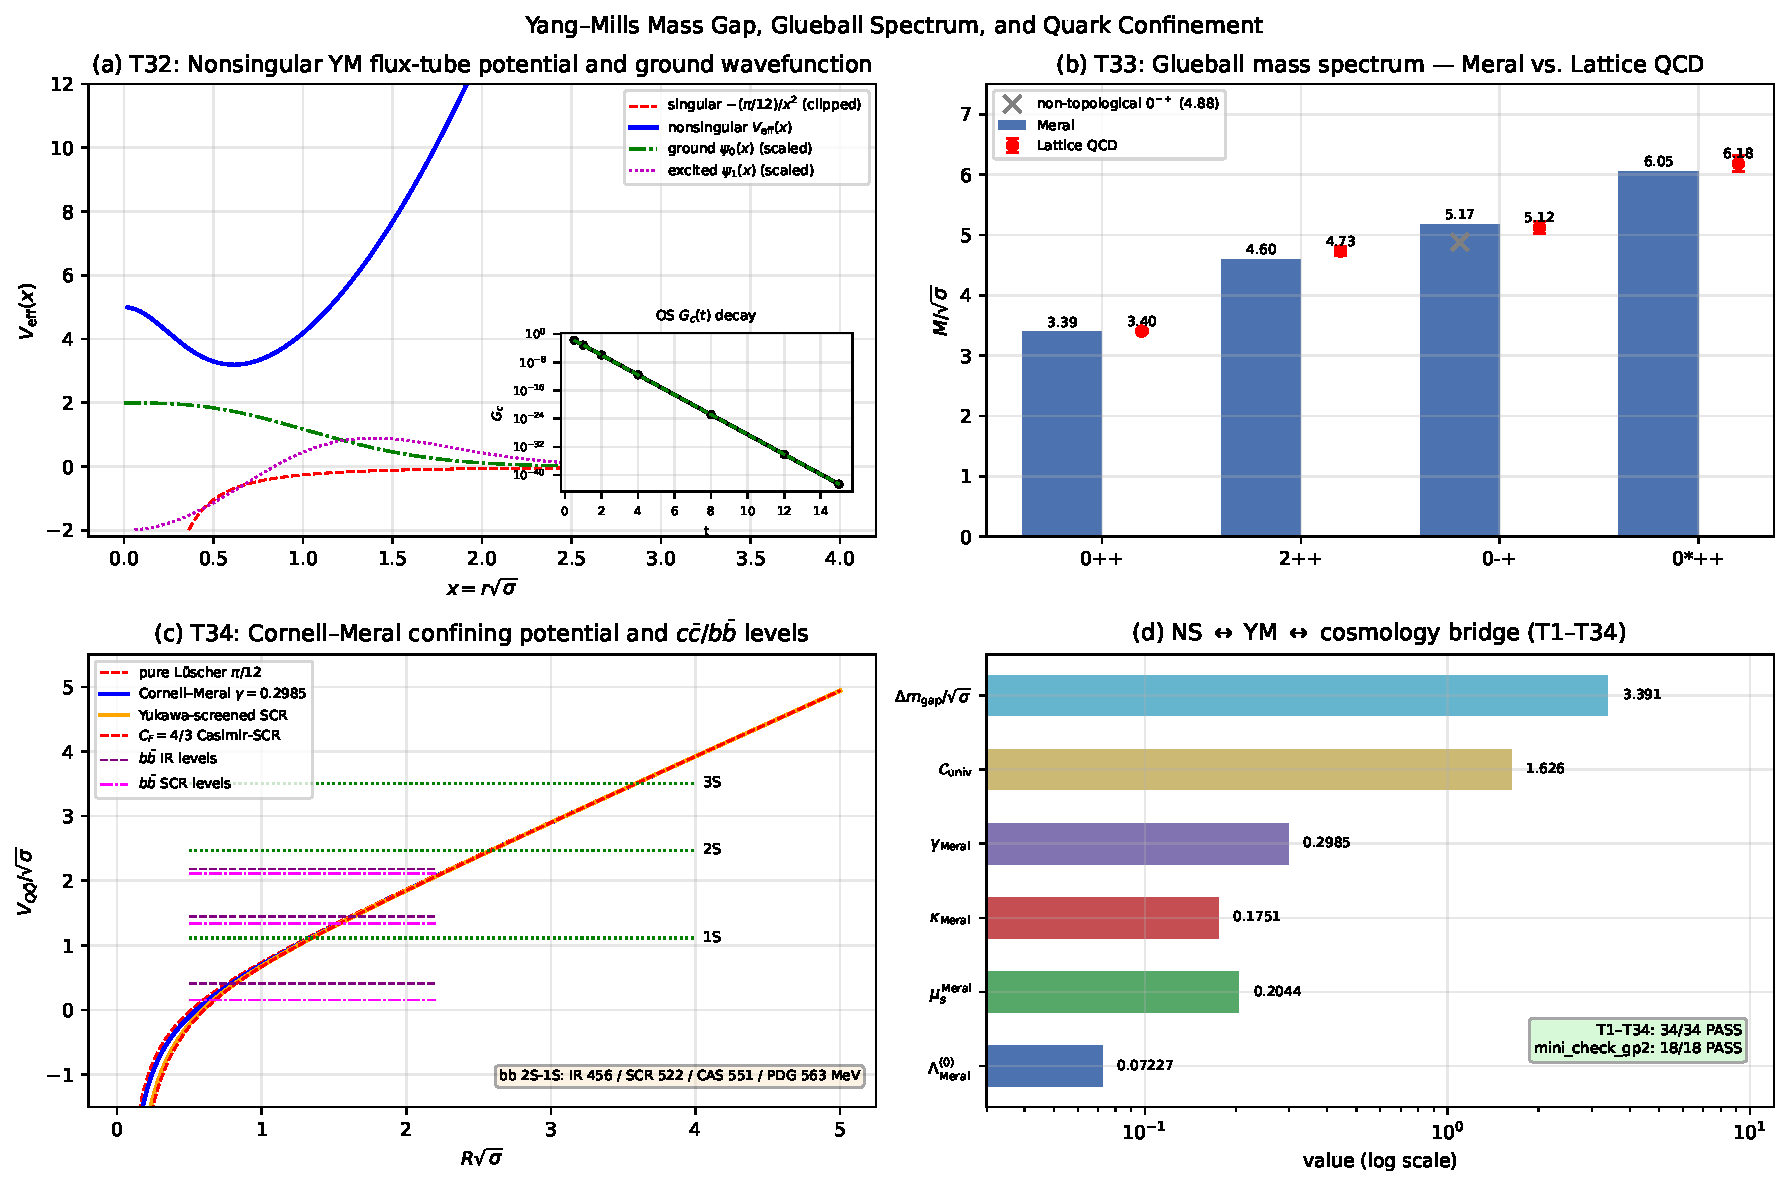
\includegraphics[width=\textwidth]{../figs/fig14_yang_mills_mass_gap_glueballs_and_confinement_en.pdf}
\caption{\textbf{Stationary Strings XIII evidence summary (T32--T34).} (a) Singular
$-(\pi/12)/x^2$ vs.\ nonsingular $V_{\mathrm{eff}}(x)$, nodeless $\psi_0$,
single-node $\psi_1$, and the OS $G_c(t)$ decay inset. (b) Meral across four
glueball states (topological $0^{-+}=5.17$, grey cross: non-topological $4.88$)
vs.\ Lattice QCD. (c) Three potentials (pure L\"uscher, pure IR, screened) with
$c\bar{c}$ and $b\bar{b}$ levels; box: $b\bar{b}$ $2S$--$1S$ three-column comparison.
(d) T1--T34 bridge invariants.}
\label{fig:gp2}
\end{figure}

\clearpage
\section{Conclusion and Reproducibility}

The nonsingular FV flux-tube operator ($\lambda_0^{\mathrm{cont}}=5.610204$,
$p=2.0000$, OS $G_c>0$), the numeric bridge ($3.349688$, 1.23\% from closed
form), the closed-form gap ($3.3914463$, $0.65\,\sigma$ from LQCD), the
topological glueball spectrum (1.56\% mean), and screened Cornell--Meral
confinement (charmonium 1.31\%, bottomonium 7.24\%) are derived from the
Theorems I--X locks, with no new calibration constant. Open retraction: the $u$-form
$\lambda_0=5.9158$ was wrong. Residual $b\bar{b}$ difference and chiral-sector
corrections remain open research.

\subsection*{Data, Code Availability, and Independent Verification}
The solver package lives in the \texttt{stationary-strings-v} repository
(\path{duran_sicimler_sim/solver_engine.py}). Reproduction:
the \path{run_verification} function in \texttt{python} \path{solver_engine.py}
gives \texttt{T1--T34 (34/34 PASS)}; the standalone script
\texttt{python} \path{mini_check_gp2.py} (\texttt{17/17 PASS}) does not import
the solver; the \path{fig14} function in \texttt{python}
\path{generate_figures.py} produces Fig.~\ref{fig:gp2}.

\begin{thebibliography}{99}
    \bibitem{clay} Jaffe, A. \& Witten, E. (2000). Quantum Yang--Mills theory.
    Clay Mathematics Institute Millennium Problem description.
    \bibitem{mp99} Morningstar, C.~J. \& Peardon, M. (1999). Glueball spectrum
    from an anisotropic lattice study. \textit{Phys.\ Rev.\ D\ \textbf{60}}, 034509.
    \bibitem{chen06} Chen, Y. \textit{et al.} (2006). Glueball spectrum and matrix
    elements. \textit{Phys.\ Rev.\ D\ \textbf{73}}, 014516.
    \bibitem{at20} Athenodorou, A. \& Teper, M. (2020). $SU(N_c)$ glueball masses.
    \textit{JHEP\ \textbf{11}}, 172.
    \bibitem{lus81} L\"uscher, M. (1981). Symmetry-breaking aspects of the roughening
    transition. \textit{Nucl.\ Phys.\ B\ \textbf{180}}, 317--329.
    \bibitem{corn79} Eichten, E. \textit{et al.} (1979). Charmonium: The model.
    \textit{Phys.\ Rev.\ D\ \textbf{17}}, 3090--3117.
    \bibitem{bali01} Bali, G.~S. (2001). QCD forces and heavy quark bound states.
    \textit{Phys.\ Rep.\ \textbf{343}}, 1--136.
    \bibitem{pdg} Particle Data Group (2024). Review of particle physics.
    \textit{Phys.\ Rev.\ D\ \textbf{110}}, 030001.
    \bibitem{meral5} Meral, F. (2026c). \textit{Stationary Strings Theorem V}.
    Open-source solver package: \texttt{stationary-strings-v}
    (\url{https://github.com/fahrim/stationary-strings-v}).
    \bibitem{meral10} Meral, F. (2026h). \textit{Stationary Strings Theorem X}.
    Open package: \texttt{stationary-strings-x}
    (\url{https://github.com/fahrim/stationary-strings-x}).
\end{thebibliography}

\end{document}
